\section{Управляемое подпространство}

Рассмотрим систему $\dot{x} = Ax + Bu$, где 
\begin{equation}
    \begin{array}{ccc}
        A = \begin{bmatrix}
            7 & -7 & 8 \\
            6 & -5 & 6 \\
            -6 & 4 & -7
        \end{bmatrix}, &
        B = \begin{bmatrix}
            -3 \\
            -1 \\
            1
        \end{bmatrix}, &
        x_1' = \begin{bmatrix}
            -8 & 3 & 0
        \end{bmatrix},
        x_1'' = \begin{bmatrix}
            -4 & 0 & 0
        \end{bmatrix},
    \end{array}
\end{equation}

\subsection{Управляемость системы}
\subsubsection{Матрица управляемости}
Найдем матрицу управляемости $U = [B, AB, A^2B]$:
\begin{equation}
    U = \begin{bmatrix} 
        \begin{array}{c|c|c}
            \begin{bmatrix}
                -3 \\
                -1 \\
                1
            \end{bmatrix} & 
            \begin{bmatrix}
                7 & -7 & 8 \\
                6 & -5 & 6 \\
                -6 & 4 & -7
            \end{bmatrix} \times 
            \begin{bmatrix}
                -3 \\
                -1 \\
                1
            \end{bmatrix} &
            \begin{bmatrix}
                7 & -7 & 8 \\
                6 & -5 & 6 \\
                -6 & 4 & -7
            \end{bmatrix}^2 \times
            \begin{bmatrix}
                -3 \\
                -1 \\
                1
            \end{bmatrix}
        \end{array}   
    \end{bmatrix}
\end{equation}
\begin{equation}
    U = \begin{bmatrix}
    3 & 36 & -183 \\ 
    -1 & 29 & -103 \\ 
    1 & -29 & 103 \\ 
    \end{bmatrix}
\end{equation}
Определим ранг матрицы управляемости:
\begin{equation}
    \text{rank}(U) = 2
\end{equation}
Так как ранг матрицы управляемости меньше размерности матрицы $A$, система не является полностью управляемой. 

\subsubsection{Управляемость собственных значений}
Определим управляемость собственных значений матрицы $A$. Для каждого собственного значения найдем матрицу Хаутуса $H_i = \begin{bmatrix} A - \lambda_i I & B \end{bmatrix}$ и определим ее ранг:
\begin{enumerate}
    \item $\lambda_1 = -1$: $H_1 = \begin{bmatrix}
        8 & -2 & 8 & -3\\
        4 & -4 & 4 & -1 \\
        -4 & 0 & -6 & 1
    \end{bmatrix}$, $\text{rank}(H_1) = 2$, собственное значение не управляемо.
    \item $\lambda_2 = -2-3j$: $H_2 = \begin{bmatrix}
        9+2j & -2 & 8 & -3\\
        4 & -3+2j & 4 & -1 \\
        -4 & 0 & -5+2j & 1
    \end{bmatrix}$, $\text{rank}(H_2) = 3$, собственное значение управляемо.
    \item $\lambda_3 = -2+3j$: $H_3 = \begin{bmatrix}
        9-2j & -2 & 8 & -3\\
        4 & -3-2j & 4 & -1 \\
        -4 & 0 & -5-2j & 1
    \end{bmatrix}$, $\text{rank}(H_3) = 3$, собственное значение управляемо.
\end{enumerate}

\subsubsection{Диагональная форма системы}
\begin{equation}
    \dot{\hat{x}} = \begin{bmatrix}
        -1 & 0 & 0 \\
        0 & -2-3j & 0 \\
        0 & 0 & -2+3j
    \end{bmatrix} \hat{x} + 
    \begin{bmatrix}
        0 \\
        \frac{1 - 9j}{2} \\ 
        \frac{1 + 9j}{2}
    \end{bmatrix} u
\end{equation}
Первое число в векторе $P^{-1}B$ равно нулю, значит, что первое состояние системы не является управляемым. 
Результаты совпали с результатами, полученными при анализе управляемости собственных значений через матрицу Хаутуса.

\subsection{Грамиан управляемости}
Найдем грамиан управляемости $P(t_1)$:
\begin{equation}
    P(t_1) = \int_{0}^{t_1} e^{At}BB^Te^{A^Tt}dt
\end{equation}
Вычислим грамиан управляемости для $t_1 = 3$ с помощью функции \texttt{gram}: 
\begin{equation}
    P(3) = \begin{bmatrix}
        23.29 & 11.16 & -11.16 \\ 
        11.16 & 6.14 & -6.14 \\ 
        -11.16 & -6.14 & 6.14 \\ 
    \end{bmatrix}
\end{equation}

Найдем собственные числа Грамиана управляемости:
\begin{equation}
   \sigma(P(3)) = \{0, 1.07, 34.49 \}
\end{equation}
Первое собственное число равно нулю, что говорит о том, что Грамиан является вырожденным и система не является полностью
управляемой. Таким образом, для дальнейшего нахождения управления необходимо использовать псведообратную матрицу. 

\subsection{Управляемое подпространство}
Выясним, принадлежат ли точки $x_1'$ и $x_1''$ управляемому подпространству:
\begin{equation}
    \begin{array}{cc}
        x_1' = \begin{bmatrix}
            -8 \\
            3 \\
            0
        \end{bmatrix}, &
        x_1'' = \begin{bmatrix}
            -4 \\
            0 \\
            0
        \end{bmatrix}
    \end{array}
\end{equation}

Для этого можно записать расширенную матрицу управляемости $U'$ и найти ранг этой матрицы:
\begin{equation}
    U' = \begin{bmatrix}
        3 & 36 & -183 & -8 \\ 
        -1 & 29 & -103 & 3 \\ 
        1 & -29 & 103 & 0 \\ 
    \end{bmatrix}
\end{equation}
\begin{equation}
    \text{rank}(U') = 3
\end{equation}

\begin{equation}
   U'' = \begin{bmatrix}
        3 & 36 & -183 & -4 \\ 
        -1 & 29 & -103 & 0 \\ 
        1 & -29 & 103 & 0 \\
    \end{bmatrix}
\end{equation}
\begin{equation}
    \text{rank}(U'') = 2
\end{equation}

Таким образом, можно сделать вывод, что точка $x_1''$ принадлежит управляемому подпространству, а точка $x_1'$ не принадлежит. В дальнейшем будем обозначать $x_1''$ как $x_1$.

\subsection{Управление системой}
Найдем управление $u(t)$, которое будет переводить систему из состояния $x(0) = 0$ в состояние $x_1 = x(t_1) = \begin{bmatrix} -8 & 3 & 0 \end{bmatrix}^T$. 
\begin{equation}
    u(t) = B^Te^{A^T(t_1 - t)}P(t_1)^{-1}x_1
\end{equation}

\begin{figure}[H]
    \centering
    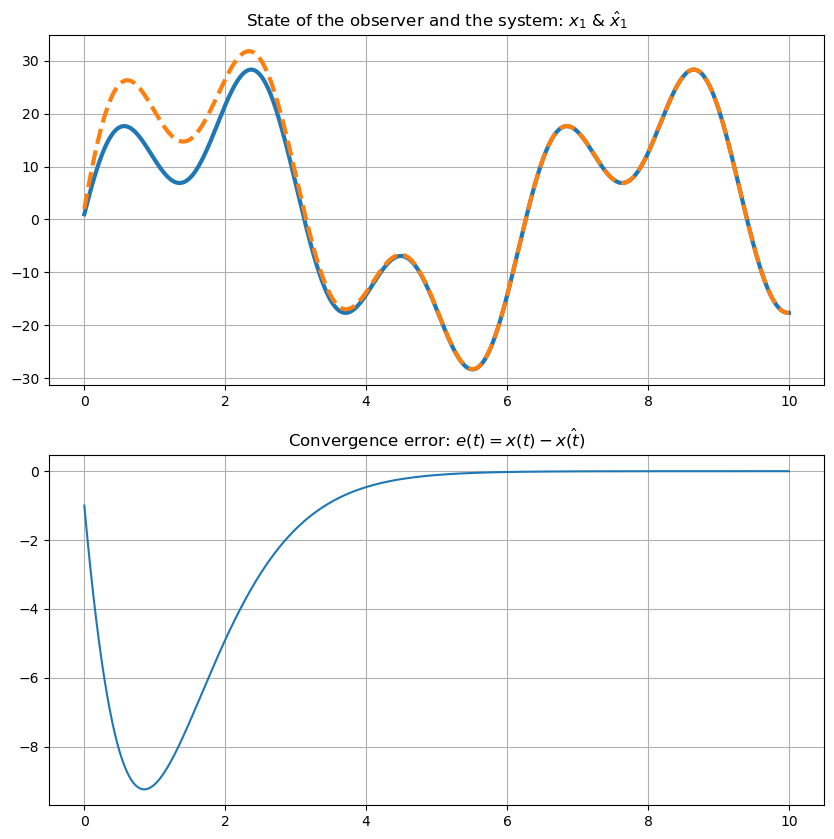
\includegraphics[width=0.9\textwidth]{../../plots/task_2_1.png}
    \caption{Управление системой}
    \label{fig:task2_control_signal}
\end{figure}

\begin{figure}[H]
    \centering
    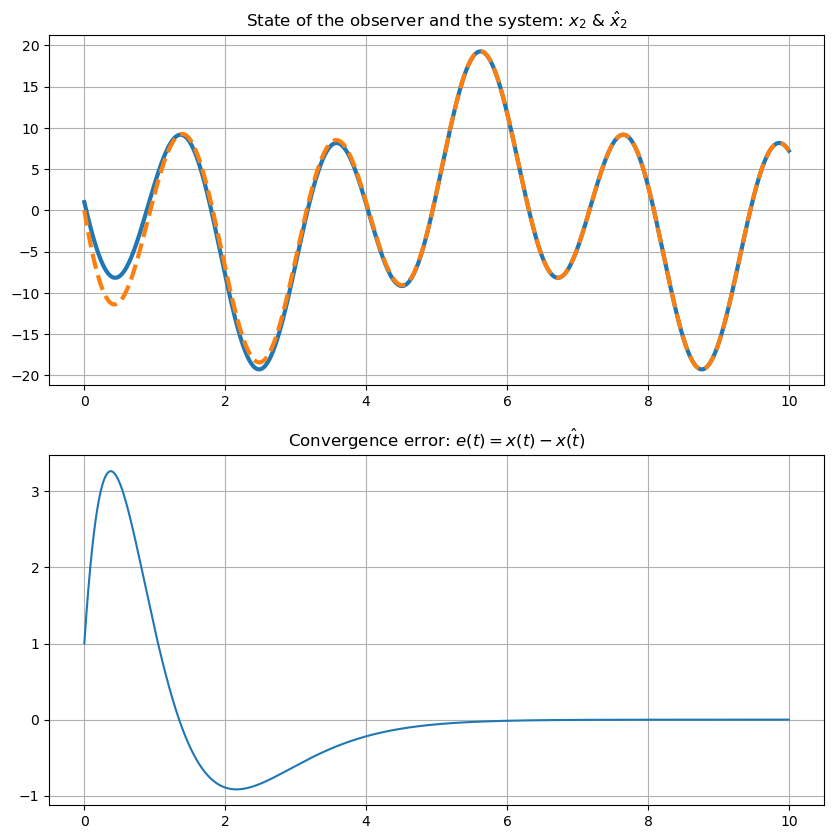
\includegraphics[width=0.9\textwidth]{../../plots/task_2_2.png}
    \caption{Состояние системы}
    \label{fig:task2_state}
\end{figure}

\subsection{Вывод}
В ходе исследования системы, представленной в данной задаче, было установлено, 
что она не является полностью управляемой. 
Это подтверждено с использованием критерия Калмана, 
а также анализом управляемости собственных значений и диагональной формы системы. 
В частности, выяснилось, что собственное число $\lambda_1 = -1$ не является 
управляемым. Дополнительно был вычислен грамиан управляемости, 
и проверка его собственных чисел показала, что одно из них равно нулю, 
что также свидетельствует о неполной управляемости системы.

Были рассмотрены две точки $x_1'$ и $x_2''$, и проведена проверка их принадлежности 
управляемому подпространству. Оказалось, что точка $x_1''$ принадлежат управляемому подпространству
в то время как точка $x_1'$ ему не принадлежит. 